\section{Register description}
\regover{
{\hyperref[spi-spi-config]{spi\_config}}&SPI configuration register
\\
\hline
{\hyperref[spi-spi-int-sts]{spi\_int\_sts}}&SPI interrupt status
\\
\hline
{\hyperref[spi-spi-bus-busy]{spi\_bus\_busy}}&SPI bus busy
\\
\hline
{\hyperref[spi-spi-prd-0]{spi\_prd\_0}}&SPI length control register
\\
\hline
{\hyperref[spi-spi-prd-1]{spi\_prd\_1}}&SPI length of interval
\\
\hline
{\hyperref[spi-spi-rxd-ignr]{spi\_rxd\_ignr}}&SPI ingnore function
\\
\hline
{\hyperref[spi-spi-sto-value]{spi\_sto\_value}}&SPI time-out value
\\
\hline
{\hyperref[spi-spi-fifo-config-0]{spi\_fifo\_config\_0}}&SPI FIFO configuration register0
\\
\hline
{\hyperref[spi-spi-fifo-config-1]{spi\_fifo\_config\_1}}&SPI FIFO configuration register1
\\
\hline
{\hyperref[spi-spi-fifo-wdata]{spi\_fifo\_wdata}}&SPI FIFO write data
\\
\hline
{\hyperref[spi-spi-fifo-rdata]{spi\_fifo\_rdata}}&SPI FIFO read data
\\
\hline
}

\subsection{spi\_config}
\label{spi-spi-config}
Address:0x4000a200
 \begin{figure}[H]
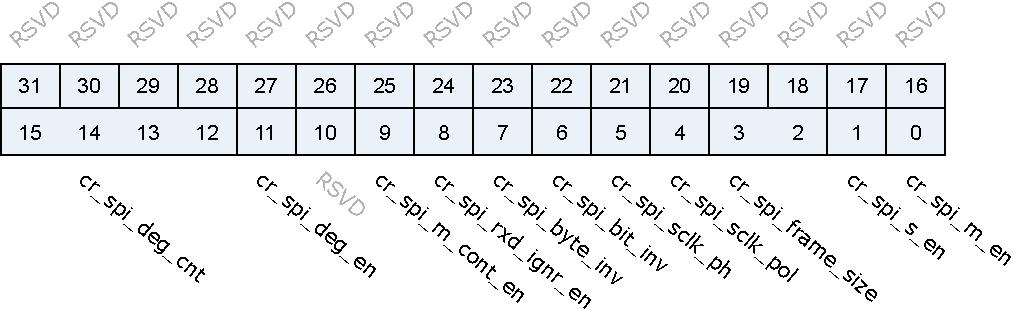
\includegraphics{spi_spi_config.pdf}
\end{figure}

\regdes{31:16&RSVD& & & \\\hline
15:12&cr\_spi\_deg\_cnt&r/w&4'd0&De-glitch function cycle count\\\hline
11&cr\_spi\_deg\_en&r/w&1'b0&Enable signal of all input de-glitch function\\\hline
10&RSVD& & & \\\hline
9&cr\_spi\_m\_cont\_en&r/w&1'b0&Enable signal of master continuous transfer mode \par 1'b0: Disabled, SS\_n will de-assert between each data frame \par 1'b1: Enabled, SS\_n will stay asserted between each consecutive data frame if the next data is valid in the FIFO
\\\hline
8&cr\_spi\_rxd\_ignr\_en&r/w&1'b0&Enable signal of RX data ignore function\\\hline
7&cr\_spi\_byte\_inv&r/w&1'b0&Byte-inverse signal for each FIFO entry data \par 0: Byte[0] is sent out first \par 1: Byte[3] is sent out first
\\\hline
6&cr\_spi\_bit\_inv&r/w&1'b0&Bit-inverse signal for each data byte \par 0: Each byte is sent out MSB-first \par 1: Each byte is sent out LSB-first
\\\hline
5&cr\_spi\_sclk\_ph&r/w&1'b0&SCLK clock phase inverse signal\\\hline
4&cr\_spi\_sclk\_pol&r/w&1'b0&SCLK polarity \par 0: SCLK output LOW at IDLE state \par 1: SCLK output HIGH at IDLE state
\\\hline
3:2&cr\_spi\_frame\_size&r/w&2'd0&SPI frame size (also the valid width for each FIFO entry) \par 2'd0: 8-bit \par 2'd1: 16-bit \par 2'd2: 24-bit \par 2'd3: 32-bit
\\\hline
1&cr\_spi\_s\_en&r/w&1'b0&Enable signal of SPI Slave function, Master and Slave should not be both enabled at the same time \par (This bit becomes don't-care if cr\_spi\_m\_en is enabled)
\\\hline
0&cr\_spi\_m\_en&r/w&1'b0&Enable signal of SPI Master function \par Asserting this bit will trigger the transaction, and should be de-asserted after finish
\\\hline

}
\subsection{spi\_int\_sts}
\label{spi-spi-int-sts}
Address:0x4000a204
 \begin{figure}[H]
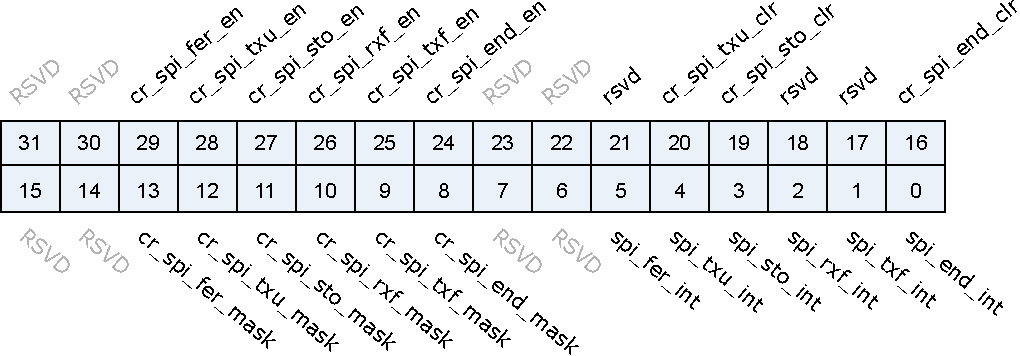
\includegraphics{spi_spi_int_sts.pdf}
\end{figure}

\regdes{31:30&RSVD& & & \\\hline
29&cr\_spi\_fer\_en&r/w&1'b1&Interrupt enable of spi\_fer\_int\\\hline
28&cr\_spi\_txu\_en&r/w&1'b1&Interrupt enable of spi\_txu\_int\\\hline
27&cr\_spi\_sto\_en&r/w&1'b1&Interrupt enable of spi\_sto\_int\\\hline
26&cr\_spi\_rxf\_en&r/w&1'b1&Interrupt enable of spi\_rxv\_int\\\hline
25&cr\_spi\_txf\_en&r/w&1'b1&Interrupt enable of spi\_txe\_int\\\hline
24&cr\_spi\_end\_en&r/w&1'b1&Interrupt enable of spi\_end\_int\\\hline
23:21&RSVD& & & \\\hline
20&cr\_spi\_txu\_clr&w1c&1'b0&Interrupt clear of spi\_txu\_int\\\hline
19&cr\_spi\_sto\_clr&w1c&1'b0&Interrupt clear of spi\_sto\_int\\\hline
18:17&RSVD& & & \\\hline
16&cr\_spi\_end\_clr&w1c&1'b0&Interrupt clear of spi\_end\_int\\\hline
15:14&RSVD& & & \\\hline
13&cr\_spi\_fer\_mask&r/w&1'b1&Interrupt mask of spi\_fer\_int\\\hline
12&cr\_spi\_txu\_mask&r/w&1'b1&Interrupt mask of spi\_txu\_int\\\hline
11&cr\_spi\_sto\_mask&r/w&1'b1&Interrupt mask of spi\_sto\_int\\\hline
10&cr\_spi\_rxf\_mask&r/w&1'b1&Interrupt mask of spi\_rxv\_int\\\hline
9&cr\_spi\_txf\_mask&r/w&1'b1&Interrupt mask of spi\_txe\_int\\\hline
8&cr\_spi\_end\_mask&r/w&1'b1&Interrupt mask of spi\_end\_int\\\hline
7:6&RSVD& & & \\\hline
5&spi\_fer\_int&r&1'b0&SPI TX/RX FIFO error interrupt, auto-cleared when FIFO overflow/underflow error flag is cleared\\\hline
4&spi\_txu\_int&r&1'b0&SPI slave mode TX underrun error flag, triggered when TXD is not ready during transfer in slave mode\\\hline
3&spi\_sto\_int&r&1'b0&SPI slave mode transfer time-out interrupt, triggered when SPI bus is idle for a given value\\\hline
2&spi\_rxf\_int&r&1'b0&SPI RX FIFO ready (rx\_fifo\_cnt > rx\_fifo\_th) interrupt, auto-cleared when data is popped\\\hline
1&spi\_txf\_int&r&1'b0&SPI TX FIFO ready (tx\_fifo\_cnt > tx\_fifo\_th) interrupt, auto-cleared when data is pushed\\\hline
0&spi\_end\_int&r&1'b0&SPI transfer end interrupt, shared by both master and slave mode \par Master mode: Triggered when the final frame is transferred \par Slave mode: Triggered when CS\_n is de-asserted
\\\hline

}
\subsection{spi\_bus\_busy}
\label{spi-spi-bus-busy}
Address:0x4000a208
 \begin{figure}[H]
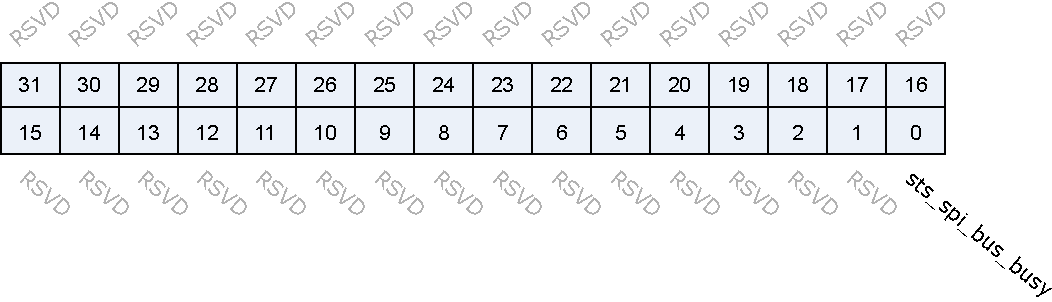
\includegraphics{spi_spi_bus_busy.pdf}
\end{figure}

\regdes{31:1&RSVD& & & \\\hline
0&sts\_spi\_bus\_busy&r&1'b0&Indicator of SPI bus busy\\\hline

}
\subsection{spi\_prd\_0}
\label{spi-spi-prd-0}
Address:0x4000a210
 \begin{figure}[H]
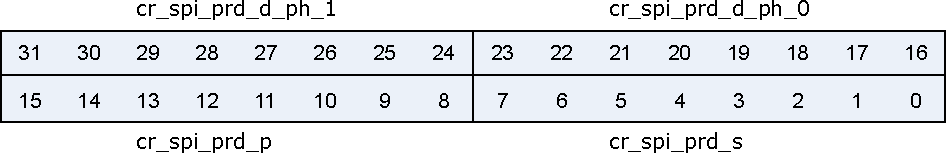
\includegraphics{spi_spi_prd_0.pdf}
\end{figure}

\regdes{31:24&cr\_spi\_prd\_d\_ph\_1&r/w&8'd15&Length of DATA phase 1 (please refer to "Timing" tab)\\\hline
23:16&cr\_spi\_prd\_d\_ph\_0&r/w&8'd15&Length of DATA phase 0 (please refer to "Timing" tab)\\\hline
15:8&cr\_spi\_prd\_p&r/w&8'd15&Length of STOP condition (please refer to "Timing" tab)\\\hline
7:0&cr\_spi\_prd\_s&r/w&8'd15&Length of START condition (please refer to "Timing" tab)\\\hline

}
\subsection{spi\_prd\_1}
\label{spi-spi-prd-1}
Address:0x4000a214
 \begin{figure}[H]
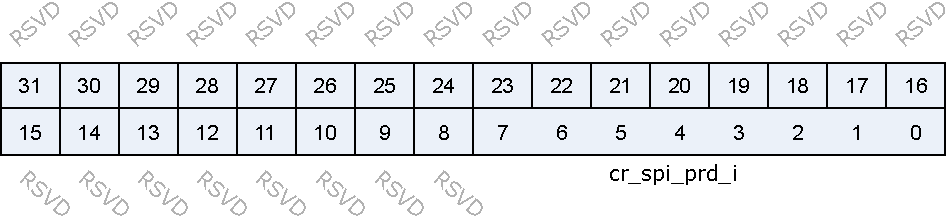
\includegraphics{spi_spi_prd_1.pdf}
\end{figure}

\regdes{31:8&RSVD& & & \\\hline
7:0&cr\_spi\_prd\_i&r/w&8'd15&Length of INTERVAL between frame (please refer to "Timing" tab)\\\hline

}
\subsection{spi\_rxd\_ignr}
\label{spi-spi-rxd-ignr}
Address:0x4000a218
 \begin{figure}[H]
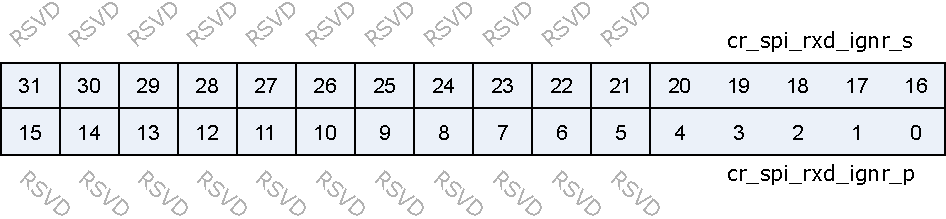
\includegraphics{spi_spi_rxd_ignr.pdf}
\end{figure}

\regdes{31:21&RSVD& & & \\\hline
20:16&cr\_spi\_rxd\_ignr\_s&r/w&5'd0&Starting point of RX data ignore function\\\hline
15:5&RSVD& & & \\\hline
4:0&cr\_spi\_rxd\_ignr\_p&r/w&5'd0&Stopping point of RX data ignore function\\\hline

}
\subsection{spi\_sto\_value}
\label{spi-spi-sto-value}
Address:0x4000a21c
 \begin{figure}[H]
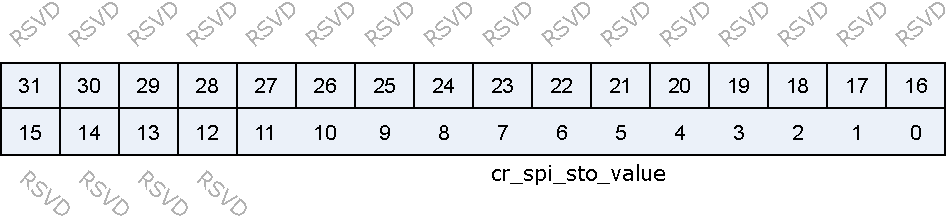
\includegraphics{spi_spi_sto_value.pdf}
\end{figure}

\regdes{31:12&RSVD& & & \\\hline
11:0&cr\_spi\_sto\_value&r/w&12'hFFF&Time-out value for spi\_sto\_int triggering\\\hline

}
\subsection{spi\_fifo\_config\_0}
\label{spi-spi-fifo-config-0}
Address:0x4000a280
 \begin{figure}[H]
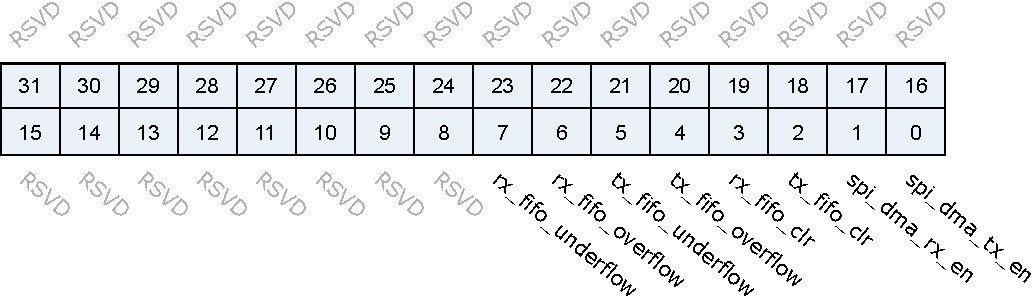
\includegraphics{spi_spi_fifo_config_0.pdf}
\end{figure}

\regdes{31:8&RSVD& & & \\\hline
7&rx\_fifo\_underflow&r&1'b0&Underflow flag of RX FIFO, can be cleared by rx\_fifo\_clr\\\hline
6&rx\_fifo\_overflow&r&1'b0&Overflow flag of RX FIFO, can be cleared by rx\_fifo\_clr\\\hline
5&tx\_fifo\_underflow&r&1'b0&Underflow flag of TX FIFO, can be cleared by tx\_fifo\_clr\\\hline
4&tx\_fifo\_overflow&r&1'b0&Overflow flag of TX FIFO, can be cleared by tx\_fifo\_clr\\\hline
3&rx\_fifo\_clr&w1c&1'b0&Clear signal of RX FIFO\\\hline
2&tx\_fifo\_clr&w1c&1'b0&Clear signal of TX FIFO\\\hline
1&spi\_dma\_rx\_en&r/w&1'b0&Enable signal of dma\_rx\_req/ack interface\\\hline
0&spi\_dma\_tx\_en&r/w&1'b0&Enable signal of dma\_tx\_req/ack interface\\\hline

}
\subsection{spi\_fifo\_config\_1}
\label{spi-spi-fifo-config-1}
Address:0x4000a284
 \begin{figure}[H]
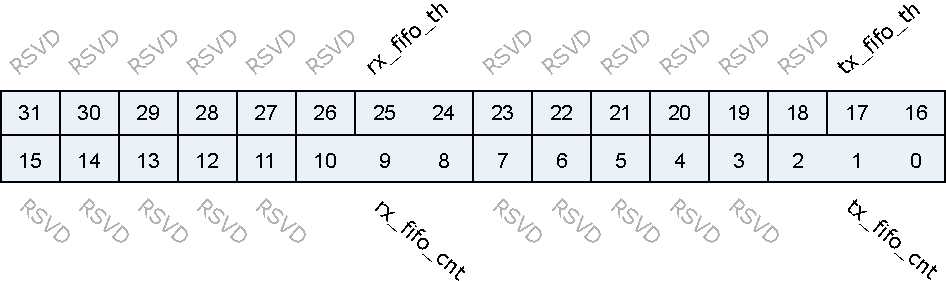
\includegraphics{spi_spi_fifo_config_1.pdf}
\end{figure}

\regdes{31:26&RSVD& & & \\\hline
25:24&rx\_fifo\_th&r/w&2'd0&RX FIFO threshold, dma\_rx\_req will not be asserted if tx\_fifo\_cnt is less than this value\\\hline
23:18&RSVD& & & \\\hline
17:16&tx\_fifo\_th&r/w&2'd0&TX FIFO threshold, dma\_tx\_req will not be asserted if tx\_fifo\_cnt is less than this value\\\hline
15:11&RSVD& & & \\\hline
10:8&rx\_fifo\_cnt&r&3'd0&RX FIFO available count\\\hline
7:3&RSVD& & & \\\hline
2:0&tx\_fifo\_cnt&r&3'd4&TX FIFO available count\\\hline

}
\subsection{spi\_fifo\_wdata}
\label{spi-spi-fifo-wdata}
Address:0x4000a288
 \begin{figure}[H]
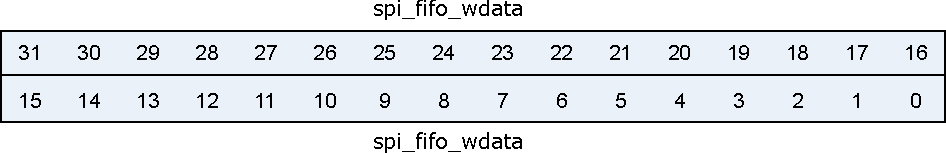
\includegraphics{spi_spi_fifo_wdata.pdf}
\end{figure}

\regdes{31:0&spi\_fifo\_wdata&w&x&\\\hline

}
\subsection{spi\_fifo\_rdata}
\label{spi-spi-fifo-rdata}
Address:0x4000a28c
 \begin{figure}[H]
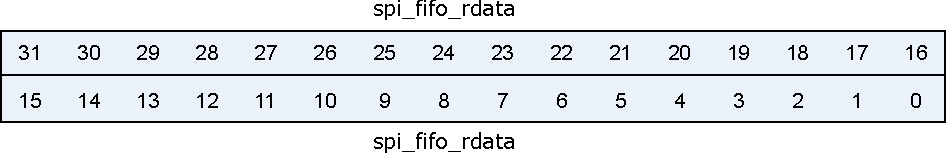
\includegraphics{spi_spi_fifo_rdata.pdf}
\end{figure}

\regdes{31:0&spi\_fifo\_rdata&r&32'h0&\\\hline

}
